\section{Backend Key Functionalities}

\subsection{User Management and Authentication}
\paragraph{}The user management module is responsible for account-related operations, including user registration, authentication, email confirmation and profile-related interactions. In addition to basic operations (CRUD) over user data, this module includes mechanisms for password handling, session management and email verification.

\subsubsection{Identity and Authentication}
\paragraph{}Authentication is handled through a token-based mechanism. The system includes the following mechanisms:
\begin{itemize}
    \item \textbf{Secure Password Handling}: Passwords are not stored in plain text. A dedicated \texttt{IPasswordEncoder} is used to generate password validation information based on hashing and salt.
    \begin{itemize}
        \item \textbf{Why Hashing and Salt?}: When a user registers or authenticates, a cryptographic hashing function transforms the plaintext password into a unique, fixed-length, and irreversible string, making it mathematically unfeasible to reconstruct the original password if the data is intercepted. To elevate this security standard, a dynamic \textit{salt}, a unique, random string is appended to each password prior to the hashing process. This ensures that even if multiple users choose the exact same password, their final stored hashes will be completely distinct from one another, effectively neutralizing dictionary attacks and pre-computed rainbow table compromises.
    \end{itemize}
    \item \textbf{Token Management}: The system manages user sessions by limiting the number of active tokens per user. When the limit is reached, the system automatically invalidates the oldest session, maintaining a balanced token lifecycle.
    \item \textbf{Email Verification}: To ensure user authenticity, the registration process triggers an asynchronous email confirmation flow. This uses a numeric code generator with a strictly defined expiration policy, enforced by the persistence layer.
\end{itemize}

\subsection{Transactional Integrity}
\paragraph{}A defining characteristic of our backend is the use of an \textbf{Atomic Transaction Manager}. Operations such as registration, password changes and email verification are executed within transactional contexts when they require multiple database changes. 
This ensures that actions such as creating a user record, generating an initial confirmation code, and updating security metadata are executed as a single unit of work. If one of the operations fails, the transaction is rolled back, avoiding partial updates. This approach is further reinforced by the \textit{OneOf} functional pattern, which forces explicit error handling for every business rule violation (e.g., duplicate emails, invalid credentials), providing predictable API responses.

\subsection{Multi-Criteria Search}
\paragraph{}The backend implements search mechanisms that allow users to query companies and creator social profiles using multiple criteria. The search logic is separated into two input models, one for creator social profiles and one for companies. Both models support pagination and filters adapted to the corresponding entity.
\begin{itemize}
    \item \textbf{Creator social profile search (\texttt{CreatorSearchInputModel}):} This model filters creator social profiles according to information associated with each specific platform profile. It processes inputs such as platform identification (\texttt{PlatformId}), username keywords (\texttt{PlatformUserName}), granular audience sizing (\texttt{FollowersCountMin} and \texttt{FollowersCountMax}), commercial budget constraints (\texttt{PriceMin} and \texttt{PriceMax}), and specific market niches (\texttt{Sectors}), all encapsulated within an optimized pagination controller (\texttt{Page} and \texttt{PageSize}). To safeguard platform reputation, this discovery layer incorporates a peer-reviewed rating system with built-in mathematical validation to strictly prevent self-rating bias.
    \item \textbf{Company search (\texttt{CompanySearchInputModel}):} Designed for creators seeking brand partnerships, this filters organizations by corporate name keywords (\texttt{Name}), active industrial or business sectors (\texttt{Sectors}), workforce scaling categories (\texttt{CompanySize}), and geographic parameters (\texttt{Countries}), utilizing matching pagination rules.
\end{itemize}

\subsection{Messaging and Conversation Architecture}
\paragraph{}The conversation module supports communication between users within the system.
\begin{itemize}
    \item \textbf{Participant Model}: Conversations support different participant types (Company vs. Creator Social Profile, Creator Social Profile vs. Creator Social Profile, Company vs. Company) through a flexible participant model, ensuring the conversation context is correctly mapped to the entity performing the action.
    \item \textbf{Conversation Management:} The system stores message state information and supports synchronization between participants.
        \begin{itemize}
            \item \textit{Message Lifecycle States:} When a participant edits a message, the system updates an \texttt{is\_edited} boolean flag to true, signaling the frontend to display an "edited" badge to both users, maintaining transparency. Similarly, message deletion utilizes a soft-delete pattern, turning the \texttt{is\_deleted} flag to true instructs the frontend to stop rendering the message content, ensuring privacy while maintaining database auditability.
            \item \textit{Unread Message Counting:} The system computes unread message counts per participant, allowing the frontend to display this information in the user interface.
            \item \textit{Background Read Synchronization:} Before a user even fully enters a conversation view, the architecture pre-evaluates and synchronizes the session state in the background against the ID of the last sent or received message. This information allows the system to determine which messages have already been read.
            \item \textit{Real-Time State Tracking:} Leveraged via native SignalR client integrations, the platform enables bidirectional web socket functionality. This updates the chat layout instantly with message states, edits, or incoming deliveries in real-time as other participants interact, completely eliminating the need for manual browser refreshes.
        \end{itemize}
    \item \textbf{Organization through Tagging}: The system allows users to create and assign private tags to conversations.Tags can be used by each user to organize conversations according to their own workflow.
    \begin{itemize}
    \item \textit{Default tags:} Out of the box, the database seeds a set of standard, industry-specific operational tags designed to map traditional partnership pipelines. These include:
    \begin{itemize}
        \item \texttt{Contacted} (Hex: \texttt{\#3498db}) — Signifies initial outreach.
        \item \texttt{Negotiating} (Hex: \texttt{\#f1c40f}) — Indicates active discussion.
        \item \texttt{Accepted} (Hex: \texttt{\#2ecc71}) — Marks a successful match and partnership agreement.
        \item \texttt{Rejected} (Hex: \texttt{\#e74c3c}) — Partnership rejection.
    \end{itemize}
    \item \textit{Custom tags:} If the default tags do not fit a user's workflow, the system allows the user to create additional tags by defining a name and a hexadecimal color code.
    \item \textit{Private visibility:} Tag assignments are private to the user who creates or assigns them. For example, when a user marks a conversation as \texttt{Negotiating} or \texttt{Rejected}, that classification is only visible to that user. The other participant does not have access to these private tags.
\end{itemize}
\end{itemize}

\subsection{History Tracking and Recommendations}
\paragraph{}The backend stores profile-view history and uses this information, together with previous search parameters, to support recommendation features. This feature allows the system to generate dashboard recommendations using information from previous profile views and search parameters, helping users discover companies or creator social profiles related to their past interactions.
\subsubsection{Recommendation Workflow}

\paragraph{}The system records profile-view events whenever a user opens a company profile or a creator social profile. This information, together with previous search parameters, is used as input for the recommendation process. The recommendation behavior differs depending on the type of entity being recommended. Figure~\ref{fig:recommendation-system} illustrates the logic behind this process.

\begin{itemize}
\item \textbf{Company recommendations:} When a user searches for companies, the search parameters can be stored and later used to recommend company profiles with similar characteristics. These characteristics may include sectors, headquarters country and company size.
\item \textbf{Creator social profile recommendations:} When a user searches for creator social profiles, the search criteria can also be stored for later use. The recommendation function can use criteria such as platform, sectors, audience size and price range to return creator social profiles related to previous searches.
\end{itemize}

\begin{figure}[H]
    \centering
    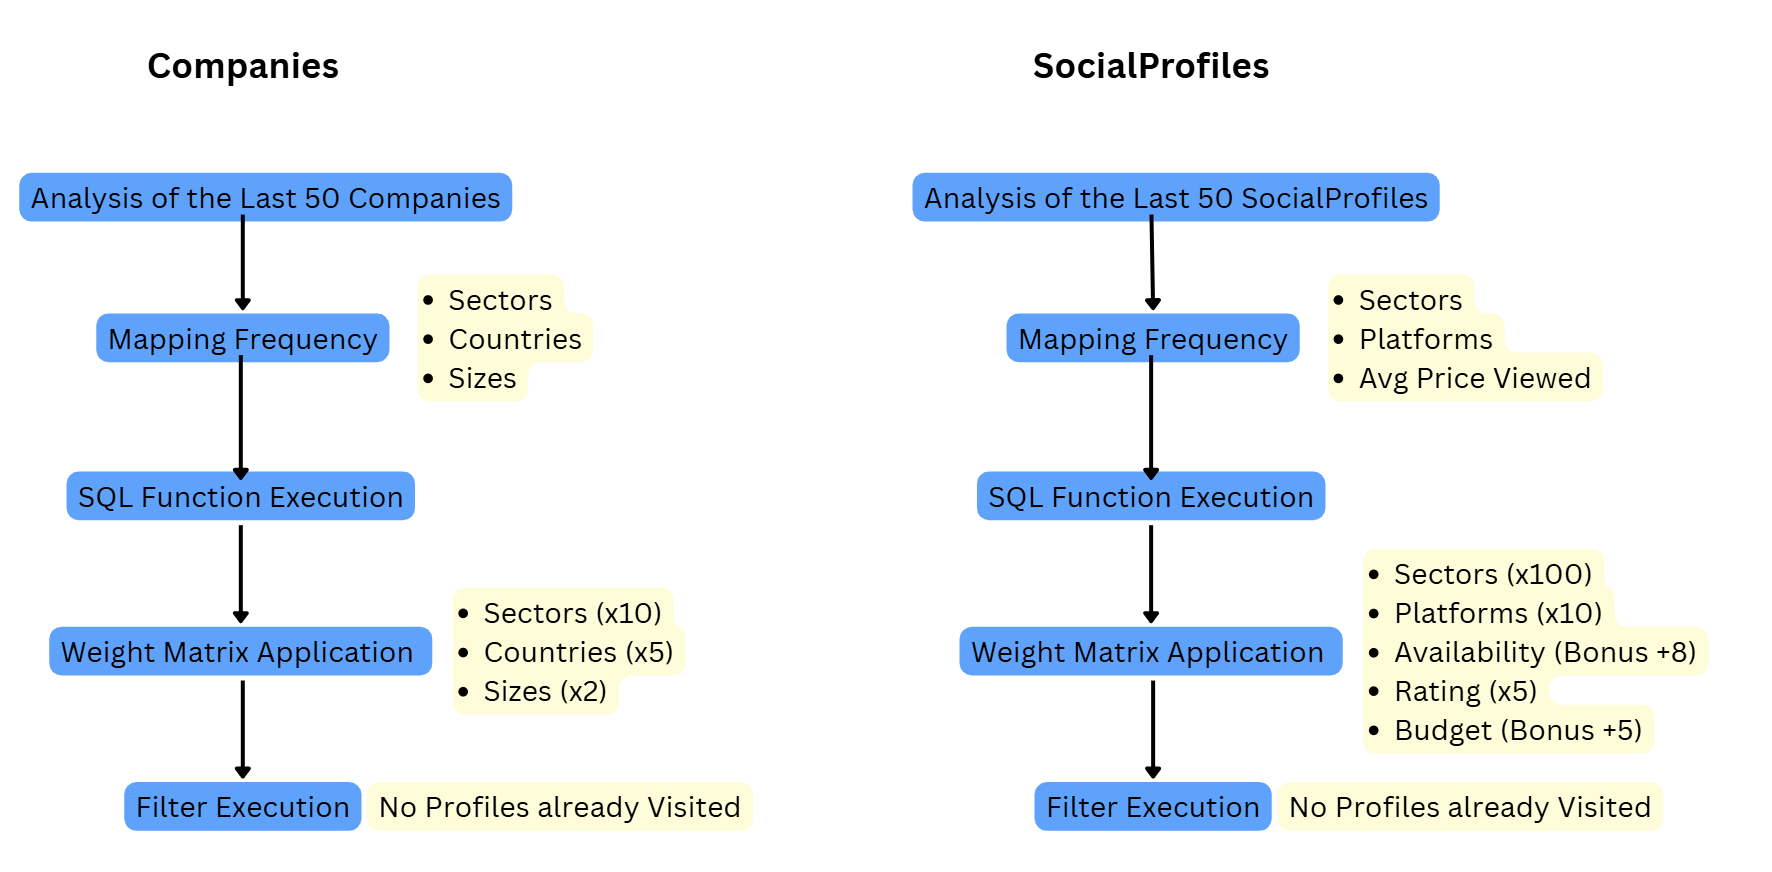
\includegraphics[width=0.95\textwidth]{./img/Recomendation_System.png}
    \caption{Recommendation System Architecture}
    \label{fig:recommendation-system}
\end{figure}


\subsection{Collaborative Coworking Framework}
\paragraph{}The Collaborative Coworking Framework enables multi-user access to a shared workspace without requiring the sharing of credentials. This mechanism establishes an operational hierarchy separating the workspace owner (administrator) from invited operators.

\subsubsection{Pipeline Integration and Context Resolution}
\paragraph{}As outlined in the request pipeline analysis, the coworker state is evaluated before the request reaches the application logic. The \texttt{RequireAuthenticationAttribute} filter and the \texttt{TokenProcessor} resolve the execution context by extracting the operator details into an \texttt{AuthenticatedCoWorker} instance, while simultaneously identifying the workspace owner as an \texttt{AuthenticatedUser}. Both objects are stored within the \texttt{HttpContext.Items} dictionary and mapped via custom model binding to be available at the controller level.

\subsubsection{Service Layer Abstraction and Audit Logging}
\paragraph{}Past the API controller layer, the underlying business services and the persistence layer operate independently of the specific identity that initiated the request. Data mutations, campaign configurations, and state updates are processed within the scope of the primary administrator's workspace identity.

\paragraph{}This design isolates core domain logic from identity validation rules, allowing the coworker to execute updates on behalf of the administrator. Because the service layer processes these changes within the context of the workspace owner, tracking individual actions within a shared workspace requires a decoupled tracking mechanism. To ensure accountability and record which physical identity performed each state modification, the architecture incorporates a dedicated Audit Logging system, as detailed in the following section.


\begin{figure}[ht]
    \centering
    \makebox[\textwidth][c]{
        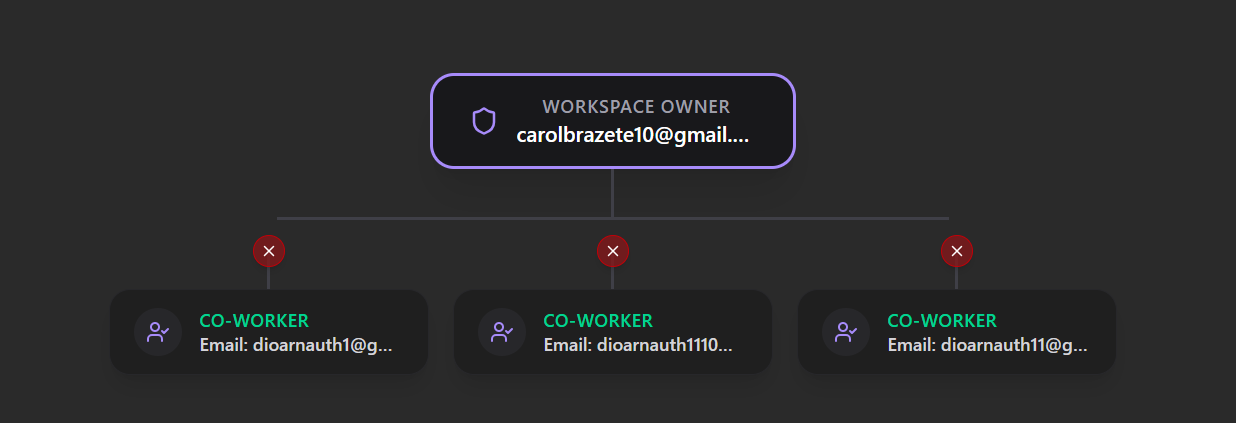
\includegraphics[width=0.95\textwidth]{./img/Team_Hierarchy_Admin.png}
    }
    \caption{Team Hierarchy - Admin Vision}
    \label{fig:team-hierarchy}
\end{figure}

\begin{figure}[ht]
    \centering
    \makebox[\textwidth][c]{
        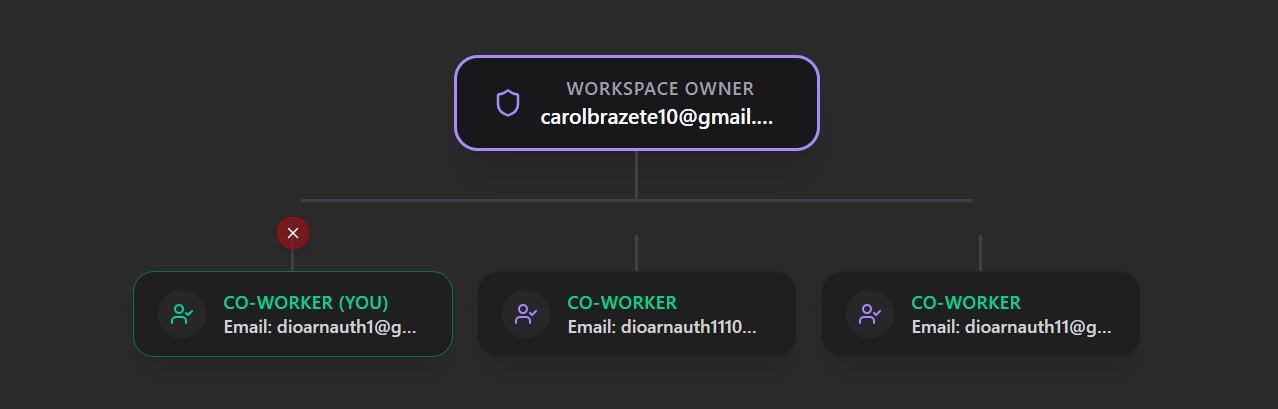
\includegraphics[width=0.95\textwidth]{./img/Team_Hierarchy_CoWorker.png}
    }
    \caption{Team Hierarchy - CoWorker Vision}
    \label{fig:team-hierarchy}
\end{figure}

\subsection{Asynchronous Audit Logging Architecture}
\paragraph{}To ensure operational accountability within shared multi-user workspaces, the platform incorporates a generalized, decoupled audit logging architecture. This framework isolates the responsibility of tracking system state changes from the primary request-execution threads, preventing administrative monitoring from introducing performance overhead or blocking user interactions.

\subsubsection{Execution Lifecycle and Queue Ingestion}
\paragraph{}The logging framework is integrated directly within the core business service layer, executing alongside the application's domain logic. When a service processes a state-changing operation, it aggregates the relevant execution metadata—such as identifiers for both the workspace owner (\texttt{UserId}) and the active operator (\texttt{CoWorkerId})—into an \texttt{AuditEntry} structure.

\paragraph{}This entry encapsulates the specific action name along with a contextual data payload resolved during the execution workflow. Once constructed, the \texttt{AuditEntry} is dispatched directly to an in-memory storage component managed by the \texttt{AuditQueue} class. This dispatch marks the transition of the audit record from the synchronous application workflow into an isolated, asynchronous processing pipeline.

\subsubsection{Asynchronous Processing and Deferred Persistence}
\paragraph{}Once an item is successfully queued, its subsequent formatting and physical database persistence are handled independently by a background infrastructure layer. The \texttt{AuditBackgroundProcessor} class operates as a long-running hosted service by extending the framework's native \texttt{BackgroundService}, continuously monitoring the queue via non-blocking asynchronous operations.

\paragraph{}Upon retrieving an entry from the queue, the processor establishes a transient dependency injection scope (\texttt{IServiceProvider.CreateScope}) to isolate the operation from any active HTTP context lifecycle. The background processing then executes the following phases:
\begin{itemize}
    \item \textbf{Reflection-Based Interpolation:} The metadata is routed through the \texttt{IAuditService} to the \texttt{AuditFormatter} utility, which uses reflection mechanisms to dynamically inspect the properties of the generic payload object.
    \item \textbf{Template Resolution:} The extracted parameters are mapped onto a static dictionary of predefined text templates, substituting structural placeholders with the actual runtime values of the operation to construct a human-readable description.
\end{itemize}
\paragraph{}Following this interpolation phase, the service instantiates the final \texttt{AuditLog} domain entity, appends a coordinated universal timestamp (\texttt{DateTime.UtcNow}), and performs a database write operation through the \texttt{IAuditRepository} to persist the historical record.